\section{Maxwellsches Fallrad}



Im ersten Teil des Experimentes wurde das Mawellsche Fallrad gemäß \cref{fig:fallrad} untersucht. Hierbei wird, anders als im freien Fall, die potentielle Energie nur zum Teil in kinetische Energie umgewandelt, da das Rad zu rotieren beginnt. Dies resultiert in einer verlangsamten Fallbewegung mit Beschleunigung $g^*$. \\

\begin{figure}[h] %{r}{0cm} wrap
	\centering
	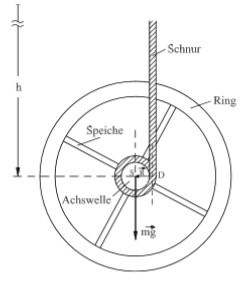
\includegraphics[width=0.5\linewidth]{res/Fallrad}
	\caption{Seitenansicht des maxwellschen Fallrades.\cite{lw}}
	\label{fig:fallrad}
\end{figure}


Aus dem geometrischen Aufbau sowie der Masse folgt das Trägheitsmoment bezüglich des Schwerpunktes, die Beschleunigung konnte direkt bestimmt werden. Der Steinersche Satz erlaubt nun Rückschlüsse auf den Abrollradius. Dieser wurde mit dem gemessenen Radius verglichen.






\subsection{Methoden}
Zur Bestimmung des Trägheitsmomentes wurde das Rad unter Benutzung eines Messschiebers mit Nonius vermessen. Alle Bestandteile wurden hierbei als Voll- oder Hohlzylinder betrachtet. Die Verdickung am Schnittpunkt der Achsen wurde nicht vermessen, zum Ausgleich wurde das Schnittvolumen der Speichen doppelt berücksichtigt. Da der Abstand der Verdickung zur Drehachse klein gegenüber dem Abstand des äußeren Ringes ist, ist davon auszugehen, dass der Unterschied zu vernachlässigen ist. Größen welche in vierter Potenz in das Trägheitsmoment eingingen wurden mehrfach gemessen, um den Einfluss von möglichen Unebenheiten des Rades auf die Ergebnisse zu verringern. Die Masse des Rades wurde mittels einer Waage bestimmt.
Anschließend wurden die Fallzeiten $t$ für fünf verschiedene Höhen $h$ je fünfmal mit einer Stoppuhr manuell bestimmt.



%\subsection{Relevante Gleichungen und Zusammenhänge}



%Für die Beschleunigung gilt\\
%$g^*= g \cdot \frac{m R^2}{J_s+m R^2}$\\
%2 Integrieren und umstellen folgt\\
%$\frac{H}{T^2}= \frac{g^*}{2}=c_{Diagramm}$\\
%Das Trägheitsmoment im  Schwerpunkt\\
%$J_s=$\\


%Aus .. folgt für den Abrollradius:\\
%$R=\sqrt{\frac{2cJ_s}{m(g-2c)}}$

